
\iffalse
\begin{figure*}[ht]
    \centering
    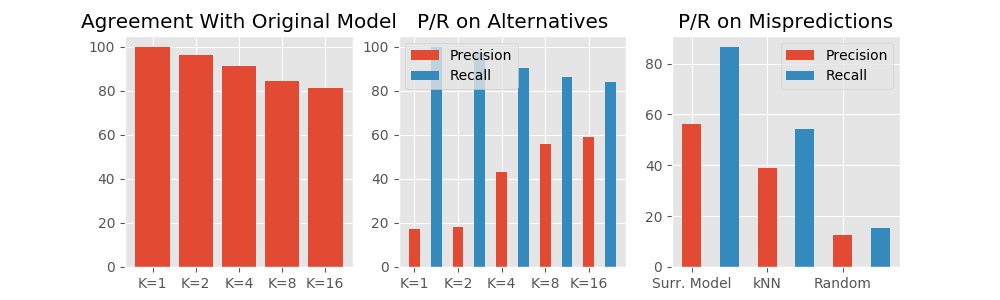
\includegraphics[width=\textwidth]{figures/result1.png}
    \caption{(A) Illustrates how a \sys  model can approximate a complex model, (B) illustrates how well this surrogate model can isolate mispredictions in terms of precision and recall, and (C) why alternative approaches do not work.}
    \label{fig:teaser}
\end{figure*}
\fi

\section{Highlighted Experiments}
This section presents key experimental results that highlight use cases where \sys models can help identify training data that cause mispredictions, 
when \sys diverges from the user's more complex model, and a comparison with alternative explanation approaches. 

\subsection{Setup}
We consider the following scenario. Suppose, the model receives a previously unseen test point that is mispredicted, can we identify the subset of training data that ``influences'' this prediction error. 
\sys returns a subset of training data using the hierarchical approximation, but we could, in principle, apply the following approaches to select relevant training data: 

\vspace{0.25em} \noindent \textbf{Nearest Neighbors: } Suppose, we measure influence purely in terms of similarity to the new data point. We could select the k-nearest neighbors in the training dataset and return them to the user. We set $k$ to be the same as number of data points returned by \sys for the new data point.

\vspace{0.25em} \noindent \textbf{Clustering: }
Another approach would be to cluster the training examples, and then return the cluster closest to the new data point. We use K-Means and set the number of clusters to 10. 

\vspace{0.25em} \noindent \textbf{Random: } Finally, as a baseline, we could randomly select training examples.  We set the number of selected examples to be the same as number of data points returned by \sys for the new data point.

\noindent \vspace{0.5em} We measure influence in the following way.
If a sample of labels of the training data outside of the selected subset are randomly perturbed, and the model is retrained, how often does the prediction change. In other words, this is a measure how ``true'' the selected neighborhood is w.r.t how the model implicitly partitions the feature space.

\subsubsection{Datasets}
We split each dataset into a training dataset $80\%$ and test dataset $20\%$. 
\stitle{Movie: } We have a dataset of movie descriptions IMDB~\footnote{ \url{ftp://ftp.fu-berlin.de/pub/misc/movies/database/}} and Yahoo~\footnote{ \url{http://webscope.sandbox.yahoo.com/catalog.php?datatype=r}}.
Each movie has a title, a short 1-2 paragraph plot description, year, rating, language, and a list of categories, and the goal is to train a model to predict whether a movie is a ``Horror'' or ``Comedy'' from the description and title.  
The total dataset has 506,244 records.
First, using TensorFlow, we trained a LSTM-based model to predict these categories. The first layer of this model computes what is called a word-embedding, where the LSTM learns a feature-space in which similar words (co-occuring) are closer together. 
The next two layers consist of dense layers that map the words from the feature-space to classification outputs.
The result is a model that achieves 93\% accuracy, which is far more accurate than simpler alternatives on a Bag-of-Words featurization (random forests 90\%, Linear SVM 81\%, Kernel SVM 85\%).

\stitle{Fraud: } ProPublica collected a dataset of corporate donations to medical researchers to analyze conflicts of interest~\cite{dollarsfordocs}. 
Records contain the PI's medical specialty, the drug brand name (null if not drug), the device brand name (null if not a device), name of pharamceutical donor, the amount donated, and whether the research is disputed.
The dataset comes with a \texttt{status} field that describes whether or not the donation was allowed under the declared research protocol.
We used a Multi-Layer Perceptron to classify disallowed donations which achieved a 82\% accuracy (random forest 81\%, Linear SVM 80\%, Kernel SVM 80\%).

\subsection{Experiments}

\stitle{Exp 1. Isolating Mispredictions } 
In the first experiment, we illustrate one benefit of \sys in terms of how it can explain predictions in terms of subsets of training data. We measure the quality of an explanation in the following way: (1) select a test data point that is mispredicted, (2) construct an explanation of this prediction by selecting a subset of training data, (3) for all examples outside of the selected subset randomly flip the labels of 25\% of the points, (4) retrain the model and observe if the test data point changes its prediction. 
We run 1000 trials of this procedure for 10 randomly sampled mispredictions and plot the results in Figure \ref{fig:isolation}. 
This metric measures how well isolated the selected neighborhood is from the other points--in other words, if the other points were changed how much would the prediction change.
The random baseline changes it prediction roughly 25\% of the time.
The clustering and the nearest neighbor approaches only consider the feature-space, not the structure of the classifier.
While they are significantly more robust than random ($\le$ 5\%) prediction changes, \sys is much more robust ($\le$ 1 \%) prediction changes.

\begin{figure}[ht]
    \centering
    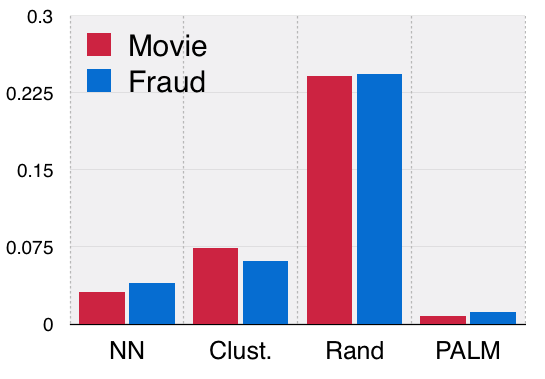
\includegraphics[width=0.7\columnwidth]{figures/isolation.png}
    \caption{\sys isolates relevant training data more effectively than baselines.}
    \label{fig:isolation}
\end{figure}

\stitle{Exp 2. Discovering other Misprediction with \sys }  
In the next experiment, we explore whether mispredictions concentrate around particular submodels. We train the models on 80\% of the dataset, and test on the remaining 20\%. We measure the fraction of mispredictions attributed to each submodel. We want to show that mispredictions concentrate around specific submodels and are not evenly distributed throughout the feature-space. Figure \ref{fig:concentrate} shows this effect when we apply our algorithm to approximate the Movie and Fraud models with $k=10$ submodels. For the Movie dataset, 70\% of the mis-predictions are attributed to a single submodel.
For the Fraud dataset, 78\% of the errors are attributed to two of the submodels.

\begin{figure}[ht]
    \centering
    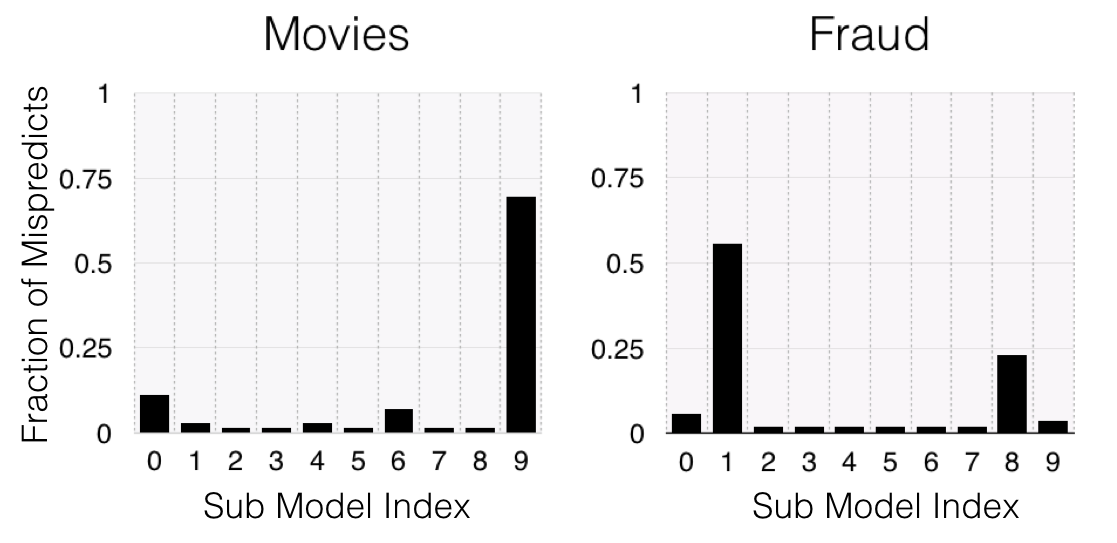
\includegraphics[width=\columnwidth]{figures/concentration.png}
    \caption{On two datasets, we show how mispredictions concentrate around specific submodels. This means there are specific regions of the feature-space most associated with mispredictions.}
    \label{fig:concentrate}
\end{figure}

\stitle{Exp 3. Agreement With the Original Model}
We now measure the agreement between the \sys model with the original model as we increasing the number of partitions $k$ (Figure~\ref{fig:agreement}, where agreement is the accuracy with respect to the original model.
We find that with $k=16$, both \sys models still retain $>90\%$ agreement with the original model.
This suggests that \sys can help developers identify more precise subsets of the training data while still trusting that the \sys models are reflective of the original model.

\begin{figure}[ht]
    \centering
    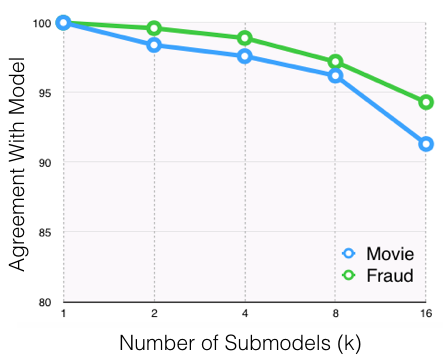
\includegraphics[width=0.6\columnwidth]{figures/agreement.png}
    \caption{On two datasets, we find that the discretized models agree with greater than 90\% accuracy with the original model. As the number of submodels increase the accuracy goes down.}
    \label{fig:agreement}
\end{figure}


\stitle{Exp 4. \sys is efficient} 
\sys can run offline during training time and queries to \sys are very efficient as it simply involves a decision tree evaluation.
\sys is explicitly designed to mimic the user's model, and the decision tree learned by the meta-model can easily be used to index or partition the training data can be indexed.
For the nearest neighbors approach, it is possible to quickly find the neighbors by using intelligent indexing structures such as KD-trees or Oct-trees.  However spatial indices are well known to have difficulty scaling to very high dimensional datasets.  In addition, finding the neighbors in a high dimensional space may simply not identify relevant results. One could apply dimensionality reduction but this would further reduce its efficacy.
On the other hand the clustering approach is much faster because it only requires querying each cluster center.
Our interesting insight is that \sys is much faster than the nearest neighbor approach, and competitive with the clustering approach in terms of run time.
Our approach returns more than 30x faster than a nearest neighbor search even when coupled with dimensionality reduction and a KD-Tree.
The clustering approach is much faster but \sys is still within the latencies needed for interactive latencies.

\begin{table}[ht!]
\centering
\caption{Run times of the different algorithms in seconds}
\label{my-label}
\begin{tabular}{lll}
Algorithm & Movie & Fraud \\ \hline
kNN & 35.61 & 22.11  \\
kNN+PCA & 12.34 & 6.97  \\
\sys & 0.334 & 0.31  \\
Clustering & 0.07 & 0.06
\end{tabular}
\end{table}